\documentclass{article}
\usepackage[final]{nips_2017}
\usepackage[utf8]{inputenc} % allow utf-8 input
\usepackage[T1]{fontenc}    % use 8-bit T1 fonts
\usepackage{hyperref}       % hyperlinks
\usepackage{url}            % simple URL typesetting
\usepackage{booktabs}       % professional-quality tables
\usepackage{amsfonts}       % blackboard math symbols
\usepackage{nicefrac}       % compact symbols for 1/2, etc.
\usepackage{microtype}      % microtypography
\usepackage{graphicx}

\newcommand\headercell[1]{\smash{\begin{tabular}[t]{@{}c@{}} #1 \end{tabular}}}

\title{Few-Shot Speaker Identification Using Masked Autoencoders and Meta-Learning}

\author{
  John Boccio \\
  Department of Electrical Engineering\\
  Stanford University\\
  \texttt{jboccio@stanford.edu} \\
  %% examples of more authors
  %% \And
  %% Coauthor \\
  %% Affiliation \\
  %% Address \\
  %% \texttt{email} \\
  %% \AND
  %% Coauthor \\
  %% Affiliation \\
  %% Address \\
  %% \texttt{email} \\
  %% \And
  %% Coauthor \\
  %% Affiliation \\
  %% Address \\
  %% \texttt{email} \\
  %% \And
  %% Coauthor \\
  %% Affiliation \\
  %% Address \\
  %% \texttt{email} \\
}

\begin{document}

\maketitle

\begin{abstract}
Speaker identification refers to the task of identifying which speaker is talking from a given set of 
speakers. With the rise of deep learning and data driven approaches to audio processing problems, new approaches can be
taken on this problem which traditionally was performed by trying to find separability between
speakers using hand-engineered feature extractors. The speaker identification problem is a very appropriate problem for meta-learning. 
Meta learning is a machine learning technique in which a model is trained to learn how to learn, allowing it to 
adapt to new tasks quickly using relatively little data. By applying meta-learning to the speaker identification problem, 
a model can be trained to learn how to recognize speakers from a small amount of audio samples from each of the speakers. 
This could be useful in scenarios where the set of possible speakers is not known in advance, or where the speakers may vary over time.
\\
\\
All of the data that was used for this paper comes from the VoxCeleb dataset \cite{DBLP:journals/corr/NagraniCZ17}. VoxCeleb
provides labeled audio data spoken from over 1,000 celebrities. These audio files are then cut into 3 second segments and 
converted into a spectrogram which will then be fed into a convolutional neural network. The final
result is a dataset with over 200,000 spectrograms, each labeled with an id that represents the celebrity that is talking.
\\
\\
The approach that this paper has taken towards applying meta-learning to the speaker identification problem is through the 
use of a prototypical network (protonet) \cite{DBLP:journals/corr/SnellSZ17}. The protonet generates an representation of a
spectrogram from one speaker which, ideally, is a far distance from the representation of a spectrogram from a different
speaker. These representations of each speaker are then used to perform classification. This paper also experiments with 
the affects of pretraining the network using a masked autoencoder \cite{DBLP:journals/corr/abs-2111-06377}.
\\
\\
Given 5 different speakers and 15 seconds of utterances from each of them, the model trained from scratch in this paper 
is able to identify who from those 5 speakers is speaking with 91.7\% accuracy. If the model is given 30 seconds of utterances
from each speaker, this accuracy increases to 95.6\%. When the model is initialized with the weights learned from the 
masked autoencoder, the accuracy decreases, implying that MAE's do not find good representations for separating speakers.

\end{abstract}

\begin{figure}
  \centering
  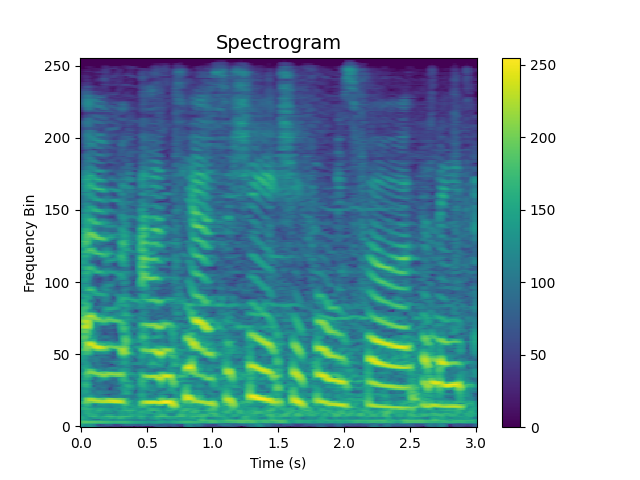
\includegraphics[width=0.6\textwidth]{Images/spectrogram_example.png}
  \caption{Spectrogram captured from 3 seconds of speech}
  \label{fig:SpectrogramExample}
\end{figure}

\section{Introduction}
The problem that this paper is solving is the problem of speaker identification; given a set of speakers, create an
algorithm to identify which one of those speakers is speaking in an audio clip. This problem has a wide variety of 
applications ranging from security, automatic speech recognition, and forensic analysis. More specifically, this paper focuses
on how to solve the speaker identification problem in a few-shot setting. Few-shot learning is an area of machine learning
which focuses on the ability of a model to learn and generalize from a small number of examples. Many cases arise in applications
where only a small amount of audio recordings from a speaker have been captured. In scenarios like this, having a few-shot
capable model is necessary. This paper explores how well a simple model can perform on the speaker identification problem when only given 3, 15, or
30 seconds of data across 3, 5, or 10 different speakers. The model used is a convolutional neural network that only
consists of convolutional layers, batch normalization layers, max pooling layers, and ReLU activation functions. The input
to this model will be spectrograms that were created from 3 seconds of speech. These spectrograms can be thought of as images
which have a label that represents an identifier for that speaker. The task of the network is to be able to identify which
speaker the spectrogram came from.

To augment few-shot learning, masked autoencoders will be used to perform unsupervised pretraining. By combining MAEs with
few-shot learning techniques, it is possible to create a model that can accurately identify speakers based on a small 
amount of input data. In this paper, we will explore the potential benefits and drawbacks of using few shot learning and
masked autoencoders for speaker identification, as well as the current state of the field and possible future directions
for research.

\section{Related work}
There are multiple ways to tackle this problem and how you do so can depend on the data that you have available and 
the use case. If all of the speakers that need to be identified are known ahead of time and that set of speakers will 
not change, then a large network could be created to perform the classification. This approach is quite fragile as it 
depends on knowing all the potential speakers ahead of time, having plently of data for each, and restricts you to 
always classifying from your entire speaker set. Another approach is to form i-vectors \cite{ivectors}. An i-vector
is a representation of an utterance that is formed by utilizing a statisical model and speech-to-text. Characteristic 
information about a speaker's voice is contained within these i-vectors which can then be applied to the speaker 
identification task. This approach works well in some scenarios but still falls short as the i-vector may not be optimal
for finding separability between speakers even though it captures the characteristics of a speakers voice well.

The disadvantages of classifying all speakers or using i-vectors can be resolved by using meta-learning. Meta-learning
enables us to selectively choose the amount of speakers we need to distinguish between and the amount of utterances we have
for each. Papers which performs similar experiements to what is done here are "Few-Shot Speaker Identification Using Depthwise
Separable Convolutional Network with Channel Attention" \cite{FewShotSpeakerIDChannelAttention} by Yanxiong Li et al. and
"Few Shot Speaker Recognition using Deep Neural Networks" by Prashant Anand et al. \cite{FewShotSpeakerRecognition}. This paper
differs from their experiments by looking at unsupervised pretraining using a masked autoencoder and utilizing a much smaller
neural network.

Autoencoders were first introduced in the book "Parallel distributed processing: explorations in the microstructure of 
cognition" \cite{ParallelDistributedProcessing}. Masked autoencoders are a derivative of autoencoders in which some of the
input to the autoencoder is hidden and it is the job of the decoder to reconstruct the missing information. Kaiming He's paper
"Masked Autoencoders Are Scalable Vision Learners" \cite{MAE} popularized this unsupervised pretraining algorithm for vision based tasks.
Many ideas from He's paper will be explored in this paper in the context of unsupervised pretraining for speaker identification.
Daisuke Nizzumi's "Masked Modeling Duo: Learning Representations by Encouraging Both Networks to Model 
the Input" \cite{MaskedModelingDuo} explores masked autoencoders and a new unsupervised reconstruction algorithm for finding representations 
of audio data. Their paper challenges MAE by stating that they do not always learn good representations. This may explain 
why this paper has found that using a MAE for unsupervised pretraining does not improve the accuracy on the speaker identification problem.

An excellent survey paper on modern day approaches to the problem of speaker identification is "Speaker Recognition Based on
Deep Learning: An Overview" \cite{SpeakerRecognitionOverview} by Zhongxin Bai and Xiao-Lei Zhang. This paper can serve as
a guide for anyone looking to experiment with different ideas related to this topic.

\begin{figure}
  \centering
  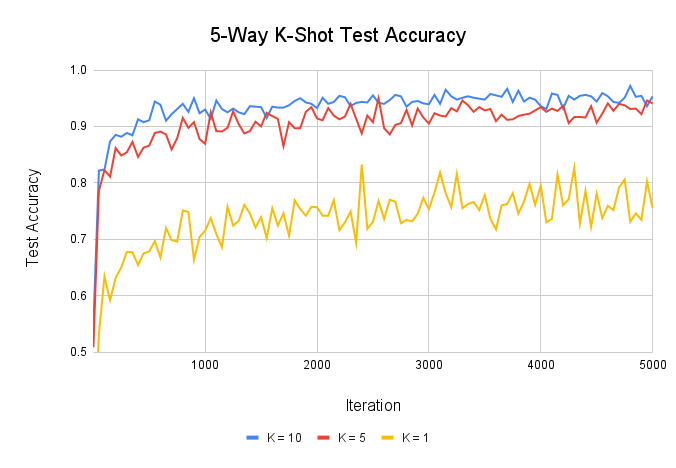
\includegraphics[width=0.8\textwidth]{Images/5-Way K-Shot Test Accuracy.png}
  \caption{Accuracy on random tasks from the test set during training with 5-way K-shot learning}
  \label{fig:FiveWayAccuracy}
\end{figure}


\section{Dataset and Features}
The dataset used for this paper consists entirely of data from VoxCeleb \cite{DBLP:journals/corr/NagraniCZ17}. The 
VoxCeleb dataset is a collection of over 150,000 utterances from 1,251 celebrities. There is also the VoxCeleb2 \cite{Chung18b} 
dataset, which has even more celebrities and utterances, but VoxCeleb1 provided enough data for the purposes of this paper.
The owners and maintainers of VoxCeleb no longer host a download for all of the audio files of the utterances but the 
links to the youtube videos with labeled timestamps is available. A tool had to be created to scrape the data off of
youtube to reconstruct this dataset. The final result is a few thousand audio files, each of which have associated labeled
timestamps that specify which celebrity was speaking.

\subsection{Audio Preprocessing}
To preprocess the audio data from the VoxCeleb1 dataset, the raw audio data was converted into a melspectrogram. A 
spectrogram is a visual representation of the frequency content of a signal over time, and it can be useful for 
analyzing the characteristics of a speaker's voice. A melspectrogram, on the other hand, represents the audio data in 
terms of mel-frequency bins, which are a nonlinear scale of frequency that is closer to the way the human ear perceives 
sound. One advantage of using a melspectrogram instead of a regular spectrogram is that it can better capture the 
characteristics of the human voice, such as the pitch and timbre. This is because the mel-frequency scale is more closely 
aligned with the way the human ear processes sound, so a melspectrogram can better represent the spectral content of speech signals.

Since all of the utterances are of different lengths, a single length had to be decided on. In this paper, the 
length that was chosen was 3 seconds. If an utterance was greater than 3 seconds, then it was split into multiple 3 
second utterances. Any utterance that was less than 3 seconds was thrown out.

The Fast Fourier Transform (FFT) was used to convert the 3 seconds of audio data into the melspectrogram. The spectrogram
was created with 256 mels, 2048 point FFTs, a hanning windowing function, and a hop length equivalent to 10 milliseconds. 
All of the audio data was downloaded at a sample rate of 16 kHz, so a 10 millisecond hop length is equivalent to 160 
samples. The audio sampling rate being 16 kHz also implies that the maximum frequency of the spectrogram is 8 kHz which 
is enough to capture most speech sounds.

Once all the utterances are converted into melspectrograms, we arrive at a labeled dataset of over 250,000 images of 
size 256 by 301. An example spectrogram can be seen in figure \ref{fig:SpectrogramExample}. This paper uses the same 
train and test split that is provided by VoxCeleb; 1,211 celebrities are in the training set and 40 celebrities are in 
the test set. The features in the melspectrograms provide the information needed to create models that can perform 
speaker identification.

\begin{figure}
  \centering
  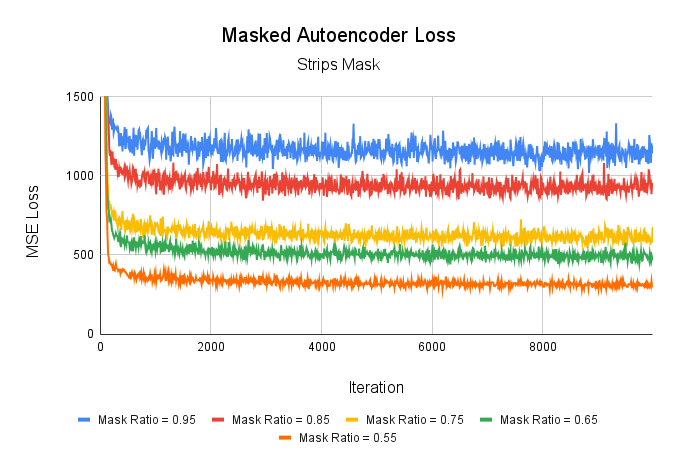
\includegraphics[width=0.8\textwidth]{Images/Masked Autoencoder Loss.png}
  \caption{Masked autoencoder MSE loss between the reconstructed output and the masked portion of the input spectrogram over iterations}
  \label{fig:MAELoss}
\end{figure}

\section{ Methods }
There are two methods used in this paper to achieve few-shot learning on the speaker identification problem. The first
method is to use protonets trained from scratch on the VoxCeleb dataset. The second method is to perform unsupervised
pretraining using a masked autoencoder and then training a protonet for few-shot learning with the weights initialized
to those learned by the masked autoencoder.

\subsection{Prototypical Network}
The data being used to identify speakers is a spectrogram of human speech. This makes makes using a convolutional neural network
a very appealing choice. A spectrogram can be treated as an image and then the CNN can be used to find features within
the spectrogram to identify the speakers. In order to perform few-shot learning with the prototypical network, the problem
needs to be formed in such a way that meta-learning can be applied, as in we want to train the network to learn how to learn
to identify speakers from a few given examples. The paper "Prototypical Networks for Few-shot Learning" \cite{DBLP:journals/corr/SnellSZ17}
outlines the theory on how to do so.

The convolutional neural network itself can be thought of as an encoder. In this paper, we used a simple 6 layer 
convlutional neural network which can be seen in table \ref{tab:CNN}. It takes as input a spectrogram and outputs a
1024-dimensional vector. When various spectrograms of a speaker are inputted into this network, the CNN should produce
similar encodings. This would imply that the encodings store information about the humans voice such as its timbre and 
pitch and not information about a particular utterance. The CNN can be driven to create such encodings by utilizing the
prototypical loss defined in "Prototypical Networks for Few-shot Learning" \cite{DBLP:journals/corr/SnellSZ17}.

When performing meta-learning, it is common to refer to the number of classes $N$ and the number of examples of each class
given as $K$, or N-way K-shot learning. When using the prototypical loss, we take our $K$ samples of each class, form the
encoding using the CNN, and average them to create a prototype for each class $\mathbf{c}_k$ as seen in equation \ref{eq:prototype}.
$S_k$ refers to all the examples for class $k$, $\mathbf{x}_i$ is the spectrogram, and $y_i$ is the speaker label.

\begin{equation}
  \mathbf{c}_k = \frac{1}{|S_k|} \sum_{\left(\mathbf{x}_i, y_i\right) \in S_k} f_\phi\left(\mathbf{x}_i\right)
  \label{eq:prototype}
\end{equation}

Once the prototypes $\mathbf{c}_k$ are created, we then classify a new speaker by creating it's encoding 
$f_\phi\left(\mathbf{x}_i\right)$ and finding which prototype $\mathbf{c}_k$ it is closest to using a distance function
$d$. This can be done with a softmax function as shown in equation \ref{eq:prototype_probability}. The network can then 
be optimized by taking negative-log probability of $p_\phi\left(y=k | \mathbf{x}\right)$ and minimizing it. The final
prototypical loss is shown in equation \ref{eq:prototypical_loss}. The number of classes $N$ and number of samples for
each class $K$ can be adjusted based on the specific problem being solved.

\begin{equation}
  p_\phi\left(y=k | \mathbf{x}\right) = \frac{\exp\left(-d\left(f_\phi\left(\mathbf{x}\right), \mathbf{c}_k\right)\right)}{\sum_{k'} \exp\left(-d\left(f_\phi\left(\mathbf{x}\right), \mathbf{c}_{k'}\right)\right) }
  \label{eq:prototype_probability}
\end{equation}

\begin{equation}
  J\left(\phi\right) = - \log \left(p_\phi\left(y=k | \mathbf{x}\right)\right)
  \label{eq:prototypical_loss}
\end{equation}

Each of the $K$ support examples for the $N$ speakers is an image of a spectrogram that consists of a 3 second utterance.
This means that there is $3.0 \cdot K$ seconds of available speech data for each of the speakers and the prototypical
network needs to learn how to identify each speaker with that amount of given data.

\subsection{Unsupervised Pretraining with Masked Autoencoders}
Autoencoders are a popular method for performing unsupervised pretraining. Autoencoders consist of an encoder and decoder
network. The encoder will take in the image of spectrogram, reduce it down to a low dimensional vector, and the decoder
will attempt to reconstruct the original spectrogram with the low dimensional vector as it's input. The idea behind this
is that if the network is able to create a low dimensional representation of the input spectrogram which can be reconstructed
into the original spectrogram with a decoder network, then that low dimensional network should hopefully contain useful 
information about what that input spectrogram had consisted of. In the context of speech processing, this low dimensional 
vector should contain information about the unique characteristics about each of the speakers voice, such as the frequency, 
intensity, and harmonic structure, as that is what is necessary to know to reconstruct the spectrograms.The weights that 
are found for the encoder can then be used to intialize the weights of the protonet which can lead to a higher accuracy 
network or faster convergence. Often, reconstructing the input image is too easy of a task for an autoencoder when the 
entirity of the input image is given. Instead, a portion of the input image, often a majority, will be masked out and it 
is the job of the autoencoder to recreate the masked out portion. This is referred to as a masked autoencoder and is 
outlined in "Masked Autoencoders Are Scalable Vision Learners" \cite{MAE} and is what will be used for pretraining in this paper.

\begin{figure}
  \centering
  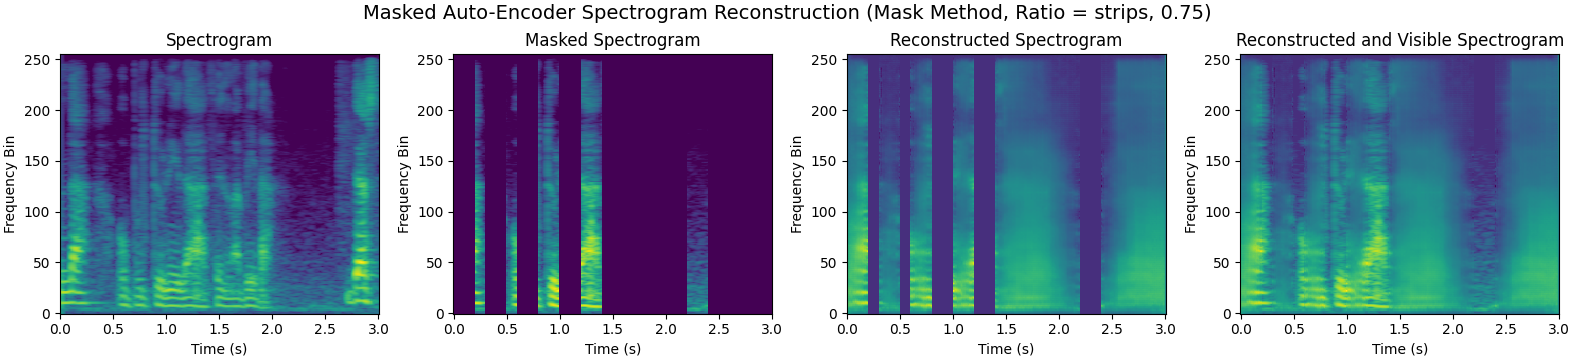
\includegraphics[width=1.0\textwidth]{Images/mae_mask_strips_mask_ratio_75_lr_005_batch_64.png}
  \caption{Masked autoencoder reconstruction on a spectrogram that had 75\% of it randomly masked using vertical strips}
  \label{fig:MAEStrips}
\end{figure}

\begin{figure}
  \centering
  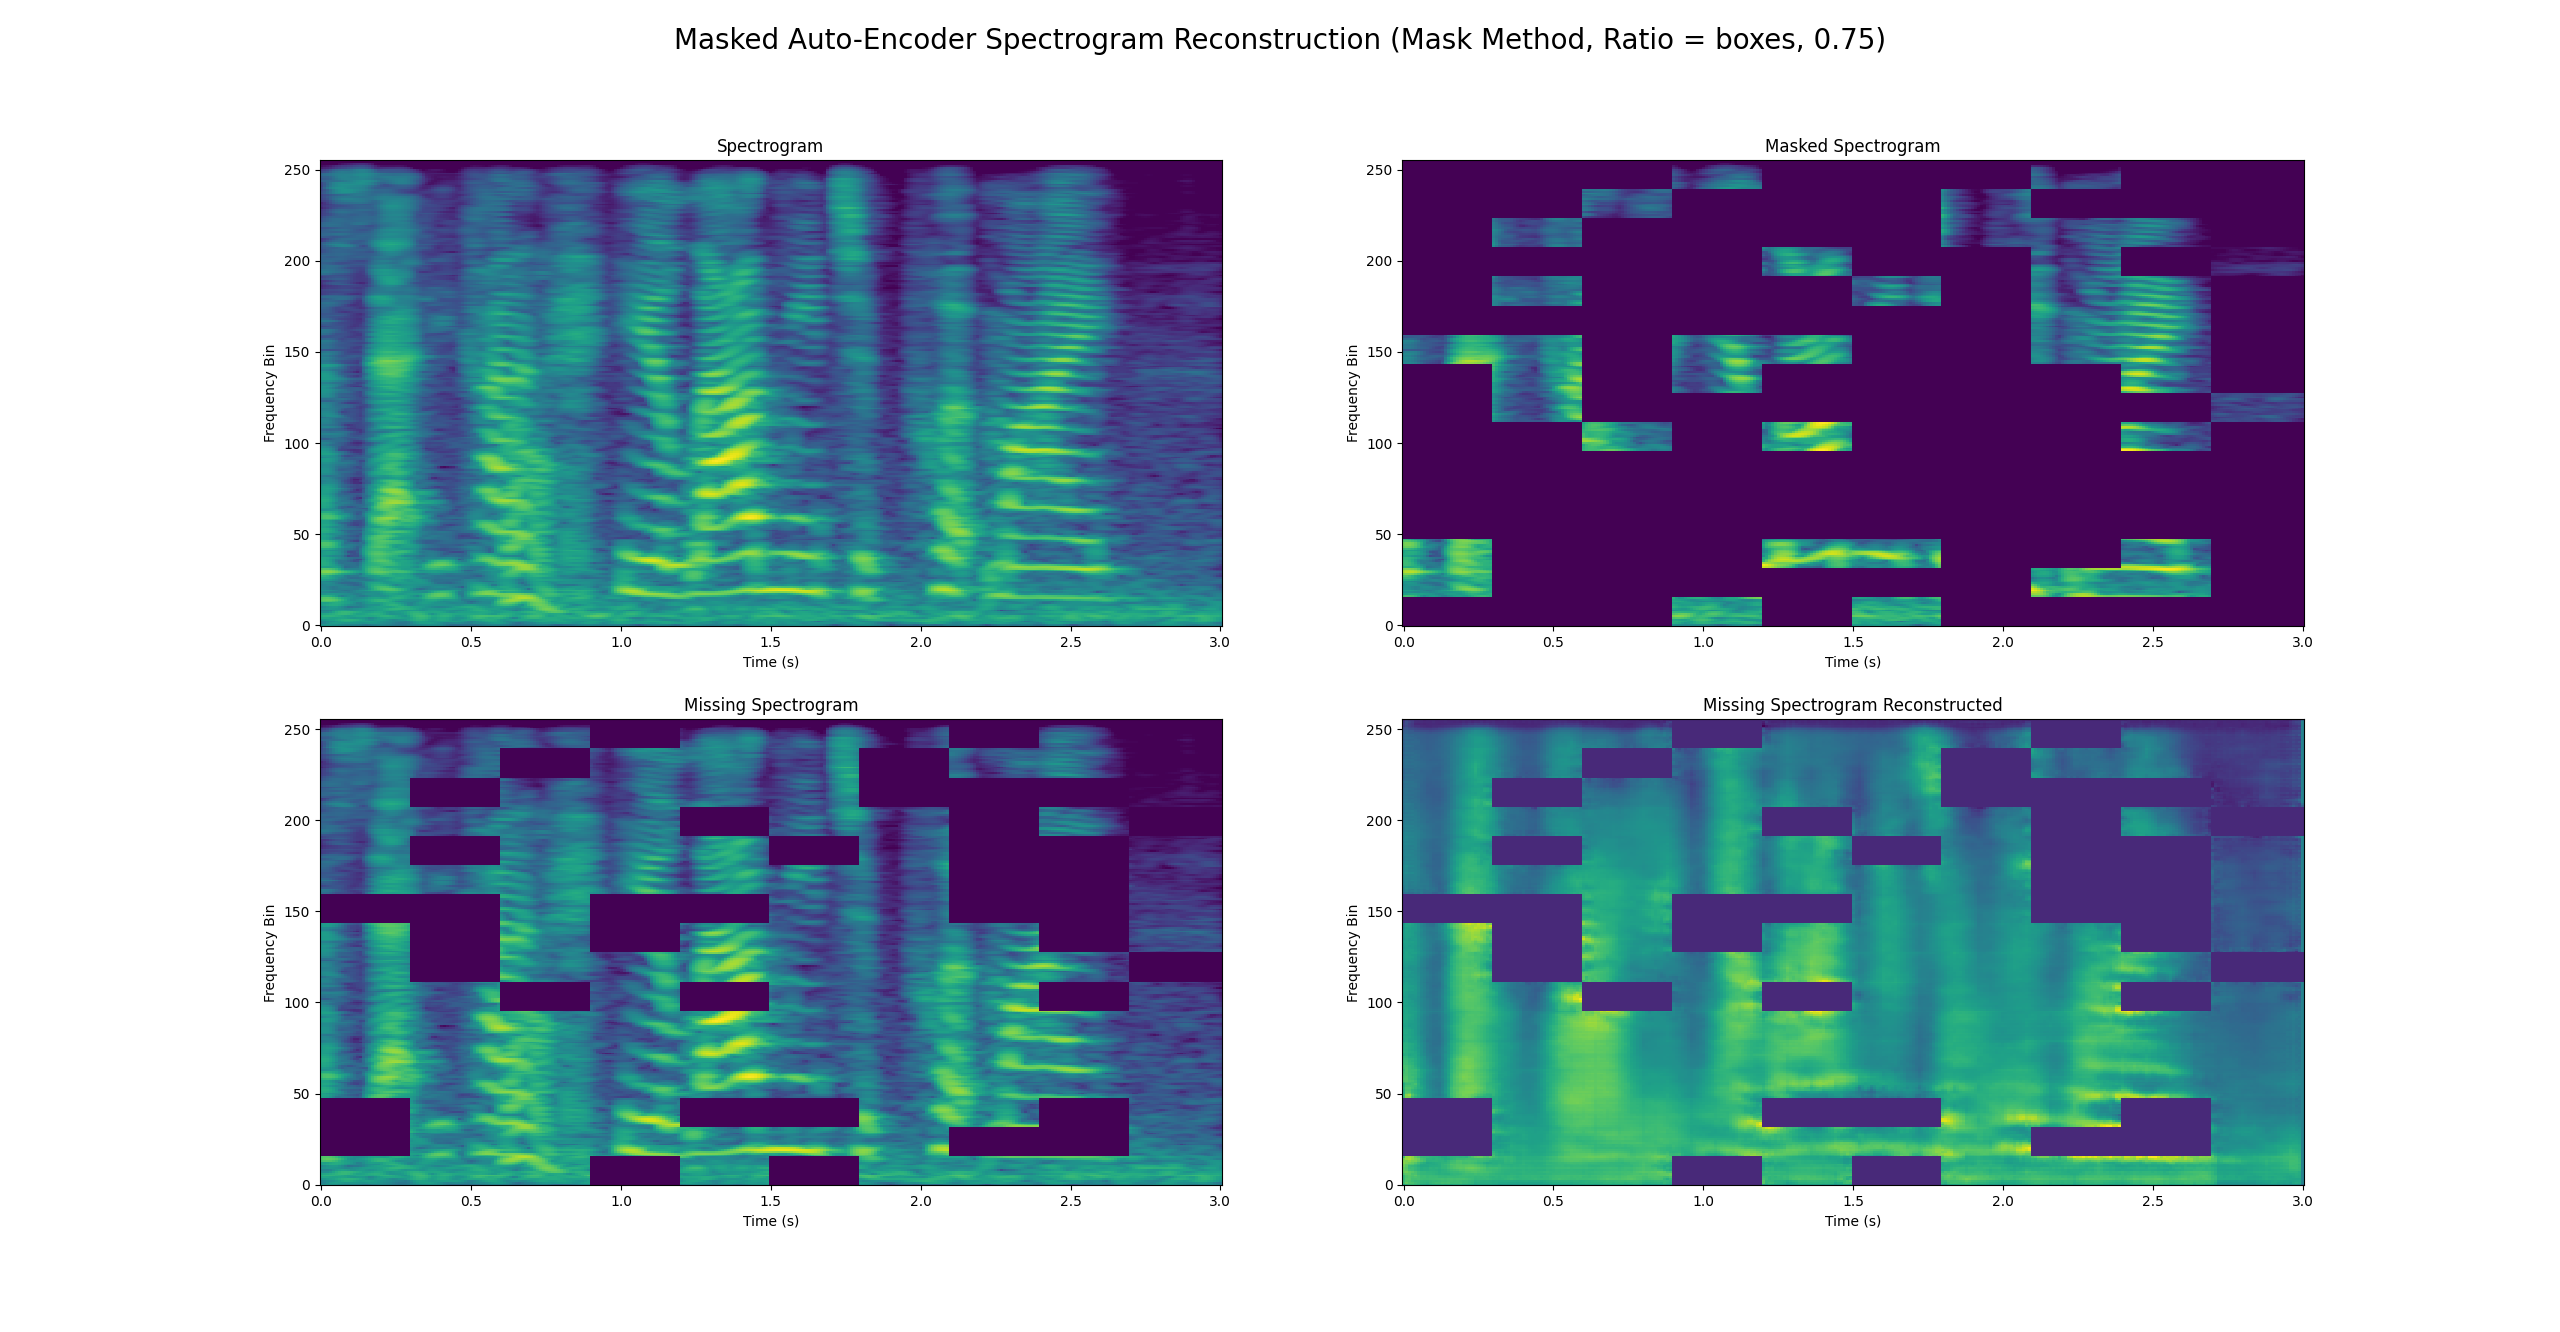
\includegraphics[width=1.0\textwidth]{Images/mae_mask_boxes_mask_ratio_75_lr_005_batch_64.png}
  \caption{Masked autoencoder reconstruction on a spectrogram that had 75\% of it randomly masked using boxes}
  \label{fig:MAEBoxes}
\end{figure}

\section{Experiments, Results, \& Discussion}
Experiments were performed on tasks that consisted of classifying utterances from 3, 5, or 10 different speakers. For
each of these tasks, 1, 5, or 10 speech examples were provided to learn from. These examples are also referred to as support set. Each
of the tasks then had 15 additional examples per speaker that were used to test how well we learned from the support 
examples. The loss is then calculated from these 15 additional examples, also known as query set, and the prototypes found from the support set.
The loss function that is used can be seen in equation \ref{eq:prototypical_loss}. The tasks were formed by first randomly selecting $N$ celebrities
from the list of celebrtiies in the dataset. Then for each of the celebrities, $K + 15$ speech utterances, which are in the form
of spectrograms, are randomly chosen to create the support and query sets. These tasks are then batched and used to train
the prototypical network whose architecture is outlined in table \ref{tab:CNN}. The accuracy on a task was defined as the
portion of the query set that was classified correctly. 

\subsection{Prototypical Network From Scratch}
The first experiments that were performed consisted of training the prototypical network from scratch (no weight initialization
from the masked autoencoder). Every 50 iterations during training, the protonet is tested on a randomly selected set of tasks from the 
test set. The amount of randomly selected test tasks was set to 4x the batch size. Figure \ref{fig:FiveWayAccuracy} shows
how the accuracy of these randomly selected test tasks throughout training.

The batch size was set to 4 when training for 3-way and 5-way classification and was set to 2 for 10-way classification.
A higher batch size would have been desirable but it was chosen to be a value which allowed the network to be trained on
the hardware that was available. The Adam optimizer was used with a learning rate of $0.001$ and was trained on $5,000$ 
tasks. This optimizer and the training hyperparameters were chosen through experimentation.

The model state was also saved every 50 iterations and at the end of training, the model with the highest accuracy on 
the random test tasks was chosen to go through $1,000$ random test tasks from the test set. The results of these chosen models
on the test set are shown in table \ref{tab:ProtonetResults} The results of this experiment show that the protonet 
performed very well at the speaker identification problem given the small amount of data. On the 5-way, 5-shot learning task,
the network described in table \ref{tab:CNN}, which only has 269,376 parameters, was able to classify the utterance correctly
with $91.7\%$ accuracy. A paper which we can compare these results against is Li et al.'s "Few-Shot Speaker Identification Using Depthwise Separable Convolutional Network with Channel Attention"
\cite{FewShotSpeakerIDChannelAttention}. Li's results show their 5-way, 5-shot network $88.74\%$ accuracy on the VoxCeleb1.
Additionally, the network had $\sim5.4x$ the amount of parameters as the one used in this paper. One possible reason as 
to why Li's network received worse accuracy with a larger network is that it is attempting to use channel attention to classify
variable length speech segments. This is different than what is performed in this paper which snips the speech segments into 
3 second intervals and performs classification on the smaller spectrograms. "Few Shot Speaker Recognition using Deep Neural Networks" \cite{FewShotSpeakerRecognition}
by Anand et al. is another paper that our results can be compared against. Anand performed transfer learning with ResNet-34, a
network with 22,354,162 parameters, on the 5-way, 5-shot speaker identification task and in doing so achieved $96.46\%$ accuracy
on VoxCeleb1. This is $\sim5\%$ more accuracy at the cost of $\sim83x$ higher compute cost. These results show us that it
is possible to perform few-shot learning on smaller networks and still achieve high accuracy.

Although the defacto test across papers has become performance on 5-way, 5-shot learning, experiments were also performed
on 3-way and 10-way. The results are as expected, the more speakers there are to classify against, the lower the accuracy.
Having more speakers increases the probability that some of them may have similar voice representations and thus leads to
the lower accuracy that is seen. Another interesting and expected result is how the $95\%$ confidence interval on the test
accuracy decreases as we increase the number of support examples. This implies that increasing the number of support examples
does not only increase the accuracy but also increases how consistent the network is at being to classify different speakers.

\begin{table}[h]
  \centering
  \begin{tabular}{@{} *{4}{c} @{}}
    \headercell{Number of Support\\Examples} & \multicolumn{3}{c@{}}{Number of Speakers} \\
    \cmidrule(l){2-4}
    & 3-Way &  5-Way & 10-Way \\ 
    \midrule
      1-Shot  & $89.4 \pm 0.004\%$  & $76.1 \pm 0.003\%$ & $67.9 \pm 0.003\%$ \\
      5-Shot  & $94.6 \pm 0.002\%$ & $91.7 \pm 0.002\%$ & $88.0 \pm 0.002\%$ \\
      10-Shot  & $96.5 \pm 0.001\%$ &  $95.6 \pm 0.001\%$ & $92.2 \pm 0.001\%$ \\
  \end{tabular}
  \caption{Results from N-way K-shot learning with the prototypical network with $95\%$ confidence interval}
  \label{tab:ProtonetResults}
\end{table}

\subsection{Prototypical Network Initialized from Masked Autoencoder}
To try to push the accuracy of the small CNN used in this paper, unsupervised pretraining with a masked autoencoder was
tried. The encoder is fed masked images of the spectrogram and produces a representation which the decoder then uses
to reconstruct the masked out portions of the input. The loss function used to compare the reconstructed output with
the masked input was the mean squared error. The MSE loss was only computed on the sections of the image that were
masked out. The encoder/decoder networks were optimized using a learning rate of 0.005 and the Adam optimizer. A batch size
of 64 was used and training was ran for 10,000 iterations, or across 640,000 spectrograms. The spectrograms were randomly
sampled during training. Multiple experiments were performed that varied how the input was masked and the portion of the 
input that was masked. 

The two masking methods that were used are referred to as "Strips" and "Boxes". With the strips method, groups of columns
of the spectrogram were masked out. In a spectrogram, each column contains the frequencies that were found at that particular
time step. Therefore, masking out a group of columns is equivalent to dropping out the audio during a short period of time
of the 3 second utterance. Each strip masked out over the input spectrogram was 10 columns wide, which equates to 100 milliseconds
of speech. The boxes method masks out rectangles of size 10 rows by 30 columns on the input spectrogram. The 10 rows represents
a portion of the frequency band that is masked out and the 30 columns masks out 300 milliseconds of speech. This method
should allow the MAE to learn how to create a representation which contains information on both the various frequency
bands of a speaker as well as how their voice changes throughout time. For both of these methods, the masks were randomly
placed on top of the input image. The portion of the input spectrogram that was masked was a hyperparameter referred to
as the mask ratio. This determines the amount of boxes and strips placed on the input image. The mask ratios that were 
tried out were 0.55, 0.65, 0.75, 0.85, and 0.95. Some examples of the masked spectrograms and their reconstruction by
the masked autoencoder are shown in figures \ref{fig:MAEStrips} and \ref{fig:MAEBoxes}.

The training loss when applying the randomly placed strips can be seen in figure \ref{fig:MAELoss}. The loss quickly decreases
for the first 100 or so iterations and then slowly decreases until the end of training. After every 250 iterations, the MAE
was tested with 10 random batches from the test set. After training was completed, the best model was selected by choosing
the one which had the lowest loss on the randomly sampled examples from the test set. Once each of the models were chosen,
the weights of the encoder were used as the initial weights of the protonet. Then, that protonet was trained to perform 
5-way, 5-shot speaker identification. The results on how well the protonet was able to perform with it's weights initialized
from the MAE's encoder are shown in table \ref{tab:ProtonetMAEResults}.

When the protonet is initialized with the MAE's encoder weights, it always performs worse than if it were trained from scratch
on 5-way, 5-shot classification. The masking method and ratio hyperparameter tuning did not make any difference as all 
of the networks converged to an accuracy that was $\sim2-3\%$ lower than that of the original 5-way, 5-shot protonet. This
conclusion supports the claim that was made in Daisuke Nizzumi's paper "Masked Modeling Duo: Learning Representations by Encouraging Both Networks to Model 
the Input" \cite{MaskedModelingDuo}. Essentially what was found was that masked autoencoders do not always find a representation
that is suitable for anything but reconstructing the input. That seems to have been what has happened with the experiments
ran for this paper as the initial weights did not increase convergence time or overall accuracy. Another possiblity is that
the VoxCeleb1 dataset provided us with a sufficient amount of data, making pretraining an unnecessary step. Training an 
encoder using a method like that in Nizzumi's paper could lead to the increase in performance that was expected.

\begin{table}[h]
  \centering
  \begin{tabular}{@{} *{6}{c} @{}}
    \headercell{Mask\\Method} & \multicolumn{5}{c@{}}{Mask Ratio} \\
    \cmidrule(l){2-6}
    & $0.55$ & $0.65$ & $0.75$ & $0.85$ & $0.95$ \\ 
    \midrule
      Strips & $87.8 \pm 0.003\%$  & $88.3 \pm 0.003\%$ & $88.6 \pm 0.003\%$ & $89.7 \pm 0.002\%$ & $88.7 \pm 0.003\%$ \\
      Boxes & $89.4 \pm 0.003\%$ & $88.3 \pm 0.002\%$ & $88.5 \pm 0.003\%$ & $89.7 \pm 0.002\%$ & $88.2 \pm 0.003\%$ \\
  \end{tabular}
  \caption{Results from 5-way 5-shot learning with the prototypical network initialized with weights from the MAE}
  \label{tab:ProtonetMAEResults}
\end{table}

\section{Conclusion and Future Work}
The field of speaker identification has been revamped by the advancement of deep learning and few-shot learning techinques.
These methods have shown up to $~20\%$ improvement in accuracy over traditional methods such as using I-vectors and probabilistic 
linear discriminate analysis \cite{ivectorPLDA}. Even the simple CNN defined in table \ref{tab:CNN} was able to achieve
$96.5\%$, $95.6\%$, and $92.2\%$ accuracy on 3-way, 5-way, and 10-way classification with just 30 seconds of audio data
for each user. Utilizing masked autoencoders for unsupervised pretraining showed to not provide any advantages. This is either
due to the MAE not learning a representation of the input which is useful for speaker identification or VoxCeleb1 providing us
enough data to the point where pretraining is not necessary. Given more computational resources, it would be great to see 
how well the network used in this paper could perform on 20-way and 50-way classification. An area which seems to continually
be a challenge for speaker identification is how to properly handle the variable length speaker utterances. The most common
and simplistic approach is to cut the utterances into smaller audio samples of a constant size, as was done in this paper.
Future work that could be explored is to utilize a transformer which can process a variable amount of spectrogram input.
Not only would this deal with the variable length issue but attention would allow for different sections of the utterance
to become interrelated and potentially lead to a higher accuracy model.

\section{Contributions}
John Boccio was the only member of the team and completed all of the work described in this report. The code for this 
project has been made public and can be found at 
\href{https://github.com/John-Boccio/SpeakerIdentificationMetaLearning}{https://github.com/John-Boccio/SpeakerIdentificationMetaLearning}.

\begin{table}[h]
  \centering
  \begin{tabular}{l|l|l}
    \textbf{Layer} & \textbf{Parameters} & \textbf{Activation Function} \\ \hline
    Input & - & - \\
    Convolutional & 16 filters, 3x3 kernel & ReLU \\
    Batch Norm. & 16 features & - \\
    Max Pooling & 2x2 pool size & - \\
    Convolutional & 32 filters, 3x3 kernel & ReLU \\
    Batch Norm. & 32 features & - \\
    Max Pooling & 2x2 pool size & - \\
    Convolutional & 64 filters, 3x3 kernel & ReLU \\
    Batch Norm. & 64 features & - \\
    Max Pooling & 2x2 pool size & - \\
    Convolutional & 64 filters, 3x3 kernel & ReLU \\
    Batch Norm. & 64 features & - \\
    Max Pooling & 2x2 pool size & - \\
    Convolutional & 64 filters, 3x3 kernel & ReLU \\
    Batch Norm. & 64 features & - \\
    Max Pooling & 2x2 pool size & - \\
    Convolutional & 64 filters, 3x3 kernel & ReLU \\
    Batch Norm. & 64 features & - \\
    Max Pooling & 2x2 pool size & - \\
    Flatten & 1024 neurons & - \\
  \end{tabular}
  \caption{Convolutional neural network used in all experiments (269,376 parameters)}
  \label{tab:CNN}
\end{table}

\bibliographystyle{plain}
\bibliography{refs}

\end{document}